\section{Deployment}

This section explains how to deploy the back-end server and all the web applications to the server.

\subsection{Back-end server}

\begin{enumerate}
    \item Download the back-end server source code to a temporary folder that does not require sudo privileges
    \item In the command line go to that folder
    \item Install dependencies - \textbf{npm install}
    \item Go to \textbf{/var/www/}
    \item Create the back-end server folder - \textbf{sudo mkdir monitor-server}
    \item Copy the back-end server source code from the temporary folder to the new folder
    \item Go back to \textbf{/var/www/}
    \item Create a secret key
    \begin{enumerate}
        \item Create a file and name it \textbf{secret.txt}
        \item Inside it write a long random string (at least 50 characters)
    \end{enumerate}
    \item Create a database configuration file
    \begin{enumerate}
        \item Create a file and name it \textbf{db.json}
        \item Copy the content from figure \ref{fig:db_config} to the new file
        \item Fill the fields with the necessary information referent to the database connection. Use the same username and password that you created when installing MySQL. Use \textbf{accessmonitor} for the database name. If the MySQL server and the web server are in the same machine the value of host should be localhost, if not, it should be the address of the MySQL server.
    \end{enumerate}
    \item Go to \textbf{/var/www/monitor-server/bin/}
    \item Start the server - \textbf{nohup node www \&}
\end{enumerate}

\begin{figure}[ht]
    \centering
    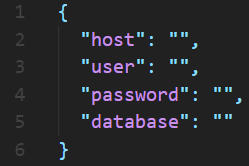
\includegraphics[width=0.5\linewidth]{lib/images/deploy/server/db_config.png}
    \caption{Database configuration JSON}
    \label{fig:db_config}
\end{figure}

\subsection{Web applications}

Before copying the web applications to the new server it is necessary to build each one of them to run in a production environment. For that follow the next steps:

\begin{enumerate}
    \item Download the application source code to a temporary folder that does not require sudo privileges folder \item In the command line go to that folder
    \item Install dependencies - \textbf{npm install}
    \item If you want to serve the applications with HTTPS follow the next substeps
    \begin{enumerate}
        \item Open the file \textbf{(...)/src/app/services/config.service.ts}
        \item Change the variable \textbf{PROTOCOL} from ``http://'' to ``https://'', line 9, figure \ref{fig:protocol_https}
    \end{enumerate}
    \item Build the application - \textbf{ng build --prod --build-optimizer}
    \item Go to the \textbf{dist} folder
    \item Open the \textbf{index.html} file
    \item Change the attribute \textbf{href} from the \textbf{base} tag (line 3 in figure \ref{fig:base_href_before}) to your application's domain (figure \ref{fig:base_href_after} shows an example with the address of the Portuguese domain)
    \item Go to \textbf{/var/www/html/}
    \item Create a new folder for the application - \textbf{sudo mkdir amp}
    \item Copy all the files from the application \textbf{dist} folder to the new created folder
    \item Inside the new folder create an access file - \textbf{sudo touch .htaccess}
    \item Copy the content from figure \ref{fig:htaccess} to the \textbf{.htaccess} file
    \item Change the \textbf{RewriteBase}, line 3, to the application's domain relative path
    \item Repeat all the previous steps for all applications
\end{enumerate}

\begin{figure}[ht]
    \centering
    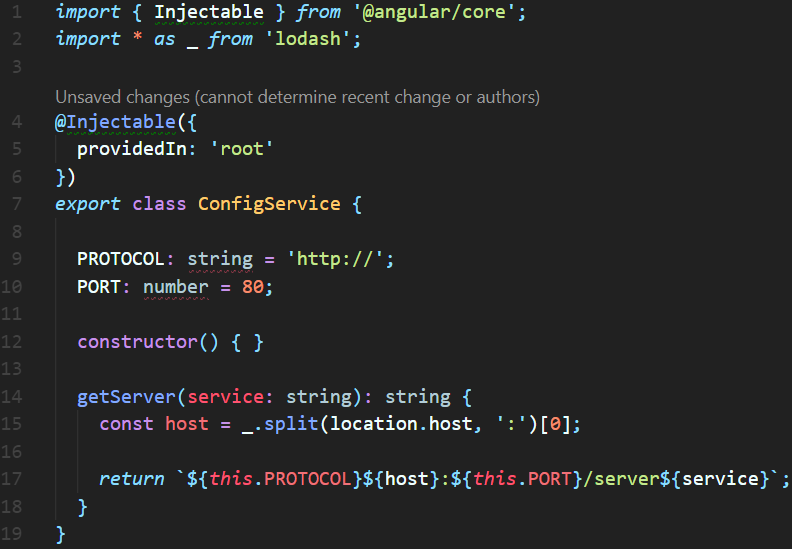
\includegraphics[width=\linewidth]{lib/images/deploy/applications/protocol_https.png}
    \caption{Change application services protocol}
    \label{fig:protocol_https}
\end{figure}

\begin{figure}[ht]
    \centering
    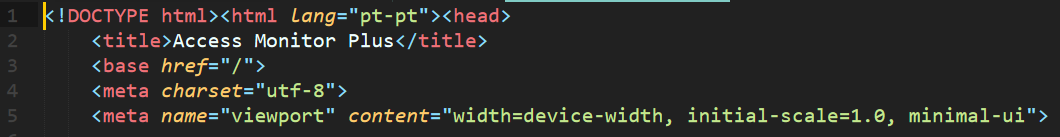
\includegraphics[width=\linewidth]{lib/images/deploy/applications/anexo_instalacao_amp_base_href_before.png}
    \caption{Base href before the modification}
    \label{fig:base_href_before}
\end{figure}

\begin{figure}[ht]
    \centering
    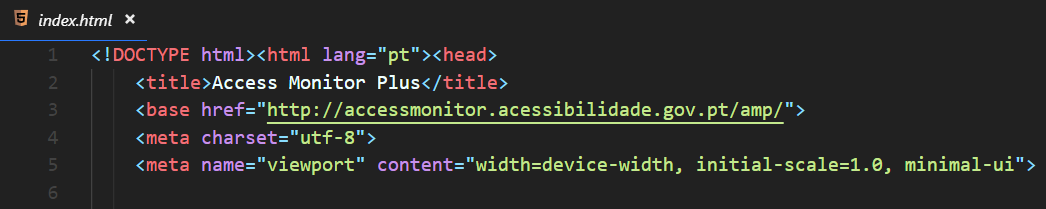
\includegraphics[width=\linewidth]{lib/images/deploy/applications/base_href.png}
    \caption{Base href after the modification}
    \label{fig:base_href_after}
\end{figure}

\begin{figure}
    \centering
    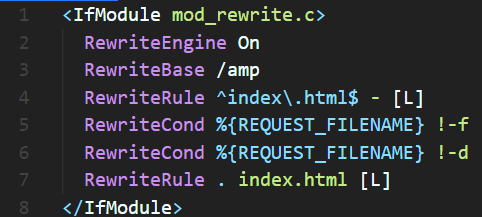
\includegraphics{lib/images/deploy/applications/htaccess.png}
    \caption{.htaccess file configuration}
    \label{fig:htaccess}
\end{figure}